\documentclass[10pt,letterpaper]{article}
\usepackage[margin=0.6in]{geometry}
\usepackage[T1]{fontenc}
\usepackage{lmodern}
\usepackage{microtype}
\usepackage{enumitem}
\setlist{nosep}
\usepackage{amsmath,amssymb}
\usepackage{booktabs}
\usepackage{tabularx}
\usepackage{xcolor}
\usepackage[colorlinks=true,urlcolor=accent,linkcolor=accent]{hyperref}
\usepackage{tikz}
\usetikzlibrary{arrows.meta}
\usepackage{titlesec}
\usepackage{needspace}

\definecolor{accent}{HTML}{1F5FA8}
\definecolor{aicol}{HTML}{C77700}
\definecolor{codecol}{HTML}{1F5FA8}
\definecolor{humcol}{HTML}{2C7A2C}

\setlength{\parindent}{0pt}
\setlength{\parskip}{2.5pt}
\setlength{\tabcolsep}{3pt}
\renewcommand{\arraystretch}{1.08}
\setlength{\emergencystretch}{2em}
\pagestyle{empty}

\titleformat{\section}{\large\bfseries\color{accent}}{}{0pt}{}[{\color{accent!40}\titlerule[0.4pt]}]
\titlespacing*{\section}{0pt}{8pt}{4pt}
\titleformat{\subsection}{\normalsize\bfseries\color{accent}}{}{0pt}{}
\titlespacing*{\subsection}{0pt}{5pt}{2pt}

\newcommand{\ct}[1]{\texttt{\small #1}}
\newcolumntype{Y}{>{\raggedright\arraybackslash}X}
\newcolumntype{L}[1]{>{\raggedright\arraybackslash}p{#1}}
\newcommand{\tabsize}{\footnotesize}

% Optional: put your name here (for example \renewcommand{\authorname}{Your Name}); it is shown under the title when non-empty.
\newcommand{\authorname}{}

\begin{document}

{\scriptsize\sffamily\bfseries\color{gray}\MakeUppercase{Tresata take-home assignment}\par}
\vspace{1pt}
{\raggedright\Large\bfseries\color{accent} Auditable Covenant Compliance: compile the contract once, compute it deterministically every quarter\par}
\ifx\authorname\empty\else{\small\textcolor{gray}{\authorname}\par}\fi
\vspace{-3pt}{\color{accent}\rule{\linewidth}{1.2pt}}

\textbf{Domain:} commercial-loan financial-covenant monitoring. \textbf{Jurisdiction:} US commercial credit agreements, using public SEC EDGAR filings. For another jurisdiction the definitions and amendment conventions would change; the architecture would not. \textbf{Evidence:} the agreement and amendment discussed below are real public documents; all borrower financial figures in the demonstration are synthetic. Cost figures are my estimates, not sourced industry benchmarks.

\textbf{What surprised me.} The ratio math is straightforward; the contractual definition is not. ``Consolidated EBITDA'' can contain bespoke add-backs and sub-caps; cash netting can be conditional; thresholds can step down; and an amendment can change which definition applies to a test date. A generic template misses these details, while an LLM-generated ratio is difficult to reproduce and audit.

%------------------------------------------------------------------
\Needspace{9\baselineskip}\section{Problem statement}
\begin{tabularx}{\linewidth}{@{}l Y@{}}
\toprule
\tabsize\textbf{Who} & \tabsize Covenant-monitoring analysts in credit administration at a mid-market lender, with a credit officer accountable for findings. \\
\midrule
\tabsize\textbf{Task} & \tabsize For each borrower and reporting period, identify financial covenants in a long credit agreement, apply amendments, extract financial inputs from statements and compliance certificates, recompute ratios under the contract's definitions, and flag breaches or thin headroom. \\
\midrule
\tabsize\textbf{Frequency} & \tabsize Quarterly (sometimes monthly). Illustrative scale: 400 borrowers, or about 1,600 tests per year. Certificates may cluster after quarter-end, creating a short review peak. \\
\midrule
\tabsize\textbf{Cost today} & \tabsize Working estimate: 4.5 hours per test, or 7,200 hours annually. At an assumed loaded rate of \$90/hour, this is about \$648,000 (approximately \$650K). These assumptions require validation with practitioners. The larger risk is a late-detected breach or a false pass. \\
\midrule
\tabsize\textbf{Out of scope} & \tabsize Waivers and reservation-of-rights decisions, legal notices, pricing and rating, non-financial covenants, equity-cure calculations, pro-forma acquisition adjustments, and real client data. The system provides decision support, not legal advice. \\
\bottomrule
\end{tabularx}

%------------------------------------------------------------------
\Needspace{9\baselineskip}\section{Solution design}
\textbf{Core idea.} Compile each agreement version into a typed, source-grounded \ct{CovenantSpec}. A human reviews and approves that specification. A deterministic engine then evaluates verified borrower facts against the approved specification each quarter. The LLM interprets unstructured contract language; it does not calculate the financial ratio or decide covenant status.

\begin{center}
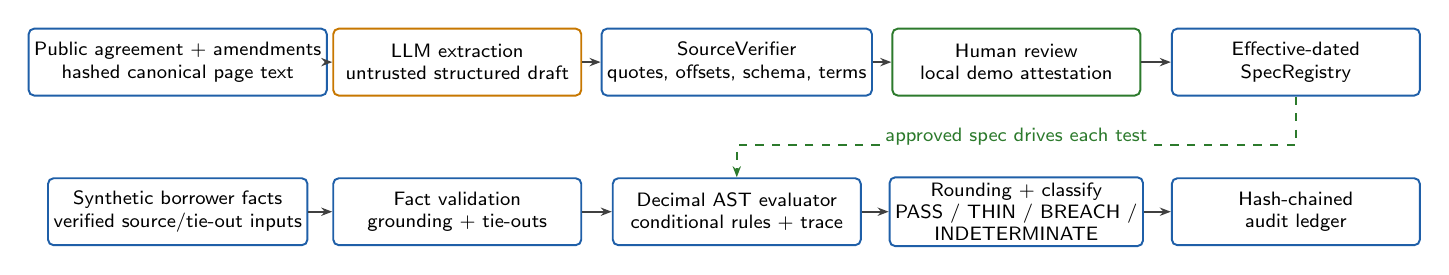
\begin{tikzpicture}[
  x=1cm,y=1cm,
  box/.style={draw,rounded corners=2pt,fill=white,line width=0.7pt,minimum width=3.15cm,minimum height=0.85cm,align=center,font=\scriptsize\sffamily,inner sep=2pt},
  cb/.style={box,draw=codecol},
  ab/.style={box,draw=aicol},
  hb/.style={box,draw=humcol},
  arr/.style={-{Stealth[length=4pt]},line width=0.7pt,draw=black!75},
  spec/.style={-{Stealth[length=4pt]},line width=0.7pt,dashed,draw=humcol}
]
\node[cb] (a1) at (1.75,0)   {Public agreement + amendments\\hashed canonical page text};
\node[ab] (a2) at (5.30,0)   {LLM extraction\\untrusted structured draft};
\node[cb] (a3) at (8.85,0)   {SourceVerifier\\quotes, offsets, schema, terms};
\node[hb] (a4) at (12.40,0)  {Human review\\local demo attestation};
\node[cb] (a5) at (15.95,0)  {Effective-dated\\SpecRegistry};
\node[cb] (b1) at (1.75,-1.9)  {Synthetic borrower facts\\verified source/tie-out inputs};
\node[cb] (b2) at (5.30,-1.9)  {Fact validation\\grounding + tie-outs};
\node[cb] (b3) at (8.85,-1.9)  {Decimal AST evaluator\\conditional rules + trace};
\node[cb] (b4) at (12.40,-1.9) {Rounding + classify\\PASS / THIN / BREACH /\\INDETERMINATE};
\node[cb] (b5) at (15.95,-1.9) {Hash-chained\\audit ledger};
\foreach \s/\t in {a1/a2,a2/a3,a3/a4,a4/a5,b1/b2,b2/b3,b3/b4,b4/b5}{\draw[arr] (\s.east) -- (\t.west);}
\draw[spec] (a5.south) -- ++(0,-0.62) -| (b3.north);
\node[font=\scriptsize\sffamily,text=humcol,fill=white,inner sep=1pt] at (12.4,-0.95) {approved spec drives each test};
\end{tikzpicture}
\end{center}
\vspace{-4pt}

\textbf{Why AI is needed.} Contract definitions are bespoke natural language with nested caps, conditions and cross-references. Retrieval and an LLM can help interpret that language and map it into a typed representation. Exact arithmetic, validation, rounding and classification remain ordinary code. This division keeps probabilistic interpretation separate from auditable calculations.

\textbf{Knowledge and lifecycle.} Contract meaning lives in a versioned, approved \ct{CovenantSpec}; source evidence lives in hash-pinned documents; bank-specific thin-headroom and sampling rules live in \ct{BankPolicy}. An amendment creates a new effective-dated specification; a restatement invalidates affected facts and dependent results; a revoked specification blocks the periods it governed until a replacement is approved. Historical records are not silently overwritten. A known but unread amendment blocks approval.

\textbf{Audit lineage.} Each result links to its ratio, AST trace, fact IDs, exact source quotations and offsets, document hash, specification hash, policy hash and engine version. The ledger records approvals, results and lifecycle events so a result can be reconstructed from its sealed inputs.

%------------------------------------------------------------------
\Needspace{9\baselineskip}\section{Workflow and implementation}
The implementation has two distinct paths. Contract extraction creates an untrusted draft that must pass provenance and structural checks before a human can approve it. Quarterly computation accepts only verified facts and an approved, effective specification.

\smallskip
\begin{tabularx}{\linewidth}{@{}l L{2.9cm} L{2.4cm} Y@{}}
\toprule
\tabsize\textbf{Step} & \tabsize\textbf{State} & \tabsize\textbf{Actor} & \tabsize\textbf{Operation and exit condition} \\
\midrule
\tabsize A1 & \tabsize INGESTED & \tabsize Code & \tabsize Hash document and preserve canonical page text and offsets. The public source corpus is reproducible from SEC EDGAR. \\
\tabsize A2--3 & \tabsize EXTRACTED & \tabsize LLM or recorded fixture & \tabsize Identify covenant language and produce structured JSON. Model output is untrusted; software derives document hashes and offsets from the cited page and quotation. \\
\tabsize A4 & \tabsize VERIFIED & \tabsize Code & \tabsize Independently verify quotations, document hashes, defined terms, AST structure, constants, threshold schedules and known amendment coverage. Reject unresolved or unsupported claims. \\
\tabsize A5 & \tabsize REVIEWED & \tabsize Human & \tabsize Display AST-generated formula, source quotations, threshold schedule, scope notes and unread terms. Reviewer explicitly approves or rejects the spec. \\
\tabsize A6 & \tabsize REGISTERED & \tabsize Code & \tabsize Verify approval attestation and register the approved specification with its effective date. \\
\midrule
\tabsize B1--2 & \tabsize FACTS & \tabsize Code and demo data & \tabsize Load synthetic financial facts, verify source spans and calculate tie-outs. Missing or unverified mandatory facts cannot produce PASS. \\
\tabsize B3--5 & \tabsize COMPUTED & \tabsize Code & \tabsize Evaluate the closed AST with Decimal arithmetic, apply contractual rounding, calculate headroom and classify the result. \\
\tabsize B6--7 & \tabsize SEALED, REVIEW & \tabsize Code and human & \tabsize Store result and trace in the hash-chained ledger; route breach, thin-headroom and indeterminate cases for human review. \\
\bottomrule
\end{tabularx}

\Needspace{6\baselineskip}\subsection{Implemented components}
\begin{tabularx}{\linewidth}{@{}L{3.0cm} Y@{}}
\toprule
\tabsize\textbf{Component} & \tabsize\textbf{Role and enforced invariants} \\
\midrule
\tabsize\ct{SourceSpan} / \ct{SourceVerifier} & \tabsize Stores document hash, page, offsets and verbatim quote. Spans carry no self-asserted verified flag; the trusted verifier checks document identity and exact text before sealing. \\
\tabsize\ct{Expr} (AST) & \tabsize Closed expression set: \ct{Lit, Input, TermRef, Sum, Diff, Mul, Div, MinOf, MaxOf, IfGt}. The LLM supplies data, never executable code. \\
\tabsize\ct{CovenantSpec} & \tabsize Numerator, denominator, defined terms, inputs, threshold steps, rounding and scope notes. Rejects undeclared inputs, unresolved or cyclic terms and invalid schedules. \\
\tabsize\ct{BankPolicy} & \tabsize Holds operational policy such as thin-headroom threshold, sampling percentage and OCR confidence requirements; policy is separately versioned and hashed. \\
\tabsize\ct{FinancialFact} & \tabsize Uses Decimal values, currency, period, scale, source evidence and grounded tie-out components. Tie-out success is derived, not supplied by the extractor. \\
\tabsize Seal + approval & \tabsize Bind verified content and approval metadata. The development signer uses local HMAC; it demonstrates tamper detection, not real-world identity authentication. \\
\tabsize Registry + ledger & \tabsize Preserve effective-dated versions, approval events, results and hash-chain history. Restatements mark dependent results stale; amendments create a new specification version. \\
\tabsize Test result & \tabsize Revalidates rounding, arithmetic, trace, headroom and classification. Staleness and previous-hash linkage are ledger concerns, not mutable result fields. \\
\bottomrule
\end{tabularx}

\Needspace{6\baselineskip}\subsection{What the prototype demonstrates, and what it does not}
\textbf{Deterministic core: implemented.} The AST evaluator performs Decimal arithmetic under an explicit 50-digit context, supports conditional rules and creates a node-level trace. The pipeline validates facts, rounds and classifies results. The registry and ledger preserve version and audit history.

\textbf{Extraction path: implemented, but not validated with live inference.} The OpenRouter provider handles timeouts, rate limits, truncation checks and requests without tools; its HTTP behaviour was tested against a fake transport. No live OpenRouter API call was made because no API key was available. The recorded provider replays \ct{data/\allowbreak extraction/\allowbreak viad\_reference\_response.json}, a reference specification manually written from the public agreement. The CLI labels this \emph{NOT A LIVE MODEL CALL}; it is not evidence of LLM extraction accuracy.

\textbf{Human approval: simulated.} The demonstration uses reviewer identifier \ct{demo.reviewer@example.com} and a local development HMAC signer. This proves that the attestation record is not altered, but does not authenticate a real credit officer. Production requires an identity-backed approval service and KMS/HSM-managed keys. No real credit officer signed the demonstration. Signed rejection records are saved locally; the CLI does not yet append them to the audit ledger.

\textbf{Reproducibility.} The public agreement pages are committed as hash-pinned canonical text; \ct{tools/\allowbreak build\_sources.py {-}{-}check} re-derives them from EDGAR. The reference specification contains 7 defined terms, 20 inputs and 4 threshold steps.

%------------------------------------------------------------------
\Needspace{9\baselineskip}\section{Public agreement and worked example}
\textbf{Source agreement.} Viad Corp (now Pursuit Attractions and Hospitality), CIK 0000884219. The original credit agreement is dated 30 July 2021 (SEC accession 0001564590-21-039835); its first amendment is dated 23 March 2022 (accession 0000950170-22-004478). The prototype uses the agreement's EBITDA and net funded indebtedness definitions (\S1.01), cash-netting cap (\S1.01), rounding rule (\S1.04), and amended leverage schedule (First Amendment \S1, restated \S7.10(c)).

\textbf{Public filings:} \href{https://www.sec.gov/Archives/edgar/data/884219/000156459021039835/vvi-ex101_28.htm}{Original Credit Agreement, SEC EDGAR} \quad|\quad \href{https://www.sec.gov/Archives/edgar/data/884219/000095017022004478/vvi-ex10_1.htm}{First Amendment, SEC EDGAR}. Filing-rendered page references used in the reference extraction: EBITDA and net funded indebtedness, pp.~17--19; unrestricted cash, p.~62; rounding, p.~64; amended covenant levels, pp.~2--3.

\Needspace{6\baselineskip}\subsection{Synthetic borrower calculation}
All borrower figures below are synthetic and expressed in USD millions. They demonstrate the contract mechanics, not an actual Viad borrower result. The example assumes no Acquisition Period is continuing.

\smallskip
\begin{tabularx}{\linewidth}{@{}l Y r@{}}
\toprule
\tabsize\textbf{Calculation} & \tabsize\textbf{Contractual operation} & \tabsize\textbf{USD m} \\
\midrule
\tabsize EBITDA before clause (d) & \tabsize $70+25+20+40+18+\min(3,5)+0+6+4+0-2$ & \tabsize 184.0 \\
\tabsize Clause (d) add-back & \tabsize $\min(40,\ 20.0\%\times184.0)=\min(40,\ 36.8)$ & \tabsize 36.8 \\
\tabsize Consolidated EBITDA & \tabsize $184.0+36.8$ & \tabsize 220.8 \\
\tabsize Netted unrestricted cash & \tabsize Revolver borrowings $25>10$; cash allowed is $\min(120,\ 50)$ & \tabsize 50.0 \\
\tabsize Net funded debt & \tabsize $(800+80+5)-\min(30,\ 50)-0-50$ & \tabsize 805.0 \\
\bottomrule
\end{tabularx}

\smallskip
\centerline{\small Leverage ratio $=805/220.8=3.645833\ldots\ \longrightarrow\ 3.646\times$}
\smallskip

\begin{tabularx}{\linewidth}{@{}l l l l Y@{}}
\toprule
\tabsize\textbf{Test date} & \tabsize\textbf{Limit} & \tabsize\textbf{Ratio} & \tabsize\textbf{Headroom} & \tabsize\textbf{Result} \\
\midrule
\tabsize 31 Dec 2022 & \tabsize 4.75x & \tabsize 3.646x & \tabsize 23.24\% & \tabsize PASS \\
\tabsize 30 Jun 2023 & \tabsize 4.00x & \tabsize 3.646x & \tabsize 8.85\% & \tabsize PASS\_THIN\_HEADROOM (illustrative 10\% BankPolicy threshold) \\
\bottomrule
\end{tabularx}

\textbf{Scope assumption.} The amendment also provides alternative leverage levels during an Acquisition Period; those alternatives are not modelled. The examples assume no Acquisition Period is continuing. A production workflow must resolve this condition from reliable borrower/event data before selecting the threshold; it must not silently assume the standard schedule when the condition is unknown.

%------------------------------------------------------------------
\Needspace{9\baselineskip}\section{Validation and risk analysis}
\textbf{Test evidence reported by the project.} 246 tests pass offline and a fresh clone reproduces them; mypy is clean across 25 source files. All 28 deliberate mutation checks are caught. No live OpenRouter call has been made.

\smallskip
\begin{tabularx}{\linewidth}{@{}L{1.9cm} Y Y@{}}
\toprule
\tabsize\textbf{Risk} & \tabsize\textbf{Failure mode} & \tabsize\textbf{Control / limitation} \\
\midrule
\tabsize Semantic error & \tabsize A real quotation is interpreted incorrectly; a consistent AST can still encode the wrong meaning. & \tabsize Source verification proves provenance, not interpretation. Human review is essential; independent historical back-testing is future work. \\
\tabsize Outdated or incomplete terms & \tabsize An amendment or side letter is missing, or a known amendment is unread. & \tabsize Known unread amendments block approval. A complete, externally confirmed amendment register remains a production requirement. \\
\tabsize Adversarial input & \tabsize Prompt injection, hidden text or fabricated figures. & \tabsize Model output is untrusted; no tools or executable code are accepted. Quotes and tie-outs are checked. OCR and hidden-text comparison are not implemented. \\
\tabsize Data and liability & \tabsize Borrower statements contain material non-public information; a demo identity is mistaken for an accountable officer. & \tabsize Prototype uses public contracts and synthetic data. Local HMAC demonstrates integrity, not identity. Production needs approved data residency, authenticated roles and KMS/HSM signing. \\
\bottomrule
\end{tabularx}

\Needspace{6\baselineskip}\subsection{Alternatives considered and next steps}
I rejected (1) a single long-context LLM call returning the ratio, because arithmetic is not reliably reproducible and source lineage is difficult to enforce; (2) per-quarter RAG chat, because it can reinterpret definitions across periods; and (3) rules/templates alone, because bespoke definitions, conditions and amendments are too varied. Deterministic rules remain in the AST execution engine.

\textbf{Before investing further.} Validate the 4.5-hour estimate and amendment-completeness process with lenders; measure live extraction on 10+ public agreements against independently reviewed specifications; and confirm tooling gaps, identity, data-residency and integration requirements. The prototype code and tests are in the public repository \href{https://github.com/Siddharth-6/covenant-audit}{github.com/Siddharth-6/covenant-audit}.

%------------------------------------------------------------------
\clearpage
\section{Appendix: What I added beyond the AI}
\textbf{Where AI helped.} I used Claude in Cursor to research the domain, challenge the architecture, draft typed models, implement the deterministic engine and extraction workflow, generate tests, and improve this brief. Claude wrote nearly all of the code. Excerpts from the prompts I gave it, verbatim from my chat logs:
\begin{enumerate}[leftmargin=1.5em,itemsep=2pt]
\item \emph{``Maintain strict separation between probabilistic nodes (LLM document ingestion, unstructured text extraction, semantic RAG) and deterministic execution engines (Pydantic validation, financial ratio math, policy rules engines).''}
\item \emph{``Do not assume that the existing implementation is correct merely because tests pass.''}
\item \emph{``The LLM should interpret the contract, but the deterministic engine must remain the sole authority for financial calculations and covenant classification.''} and \emph{``Do not simulate an LLM call while claiming that a real model was used.''}
\end{enumerate}

\textbf{What the AI got wrong, and what I required it to fix.}
\begin{itemize}[leftmargin=1.4em,itemsep=2pt]
\item \emph{Unsourced precision.} Claude proposed precise-looking cost figures (4.5 hours per test, \$650K a year). They are assumptions; I kept them labelled as my estimates and made practitioner validation a next step.
\item \emph{Defects the AI disclosed.} Claude's first implementation hardcoded the 10\% thin-headroom threshold, trusted a caller-supplied tie-out \texttt{passed} flag and a self-declared \texttt{verified} flag, and validated results in one direction only. After reading its own limitations list, I made fixing each a requirement and told it not to weaken existing tests; they became a versioned \ct{BankPolicy}, derived tie-outs, a trusted verifier with sealed content, and a result validator that re-derives classification.
\item \emph{A gap the AI found in its own fix.} While writing a prompt-injection test, Claude noticed tie-out components were still the extractor's word; each must now be a quoted, summed source line.
\item \emph{Designs ruled out.} LLM-generated Python for calculations (I instructed that the LLM must not generate executable code) and LLM self-reported confidence as a routing signal, because uncalibrated confidence correlates poorly with mathematical precision.
\item \emph{Bugs the tests exposed, fixed by the AI.} A canonicaliser that mis-paired nested quotes, a clause search that ran out of budget before the cash definition, and a false-positive ``constant denominator'' check. An old import-ban test that the new download code correctly broke was narrowed with a documented reason, not deleted.
\end{itemize}

\textbf{What came from me.} I set the problem (commercial-loan covenant monitoring) and the constraints: a strict boundary between probabilistic extraction and deterministic computation; the four audit questions (where knowledge lives, lineage, weakest link, three rejected alternatives); and a four-page limit with this appendix. I required a real public SEC agreement rather than invented clauses, and that a missing or unread amendment never be treated as absent. I directed the hardening phase (listing the defects to fix) and required that no replayed or simulated model call be presented as live, that the development signer be kept apart from production KMS signing and not described as identity authentication, and that implemented, simulated, production and unimplemented items be kept separate. I then reviewed this brief against the repository and had claims I could not stand behind corrected. The compile-once architecture, the choice of the Viad agreement and the conditional AST operation were proposed by Claude; I reviewed and accepted them.

\textbf{Important disclosure about the demonstration.} The repository's \ct{viad\_reference\_response.json} was manually written from the public agreement text. The recorded provider replays that reference and is explicitly labelled \emph{NOT A LIVE MODEL CALL}. The OpenRouter adapter is implemented and tested against a fake transport, but no live API call was made because no API key was available. The demo approval by \ct{demo.reviewer@example.com} is simulated and is not a real credit officer's sign-off. The prototype therefore demonstrates the extraction, verification, review and calculation interfaces, but does not establish live-model extraction accuracy or production identity authentication.

\textbf{One concept I can defend without AI: determinism is not semantic correctness.} For the synthetic example, the contract-capped EBITDA is $184.0+\min(40.0,\ 0.20\times184.0)=220.8$ million. Net funded indebtedness is 805 million, giving a ratio of $805/220.8=3.645833\ldots$, rounded to $3.646\times$ under the agreement's three-decimal, ties-up rule. The engine can reproduce this result exactly from the approved AST and verified inputs. But it cannot prove that the AST correctly represents the legal meaning of the agreement. A real quotation can be grounded and still be misunderstood. That is why semantic review, amendment completeness and independent validation remain critical.

\medskip
{\footnotesize\textcolor{gray}{All borrower amounts and borrower scenarios in this brief are synthetic. Public contract sources are cited above. Prototype limitations are stated explicitly; no live LLM inference or real credit-officer approval is claimed.}}

\end{document}
